% -- Encoding UTF-8 without BOM
% -- XeLaTeX => PDF (BIBER)

\documentclass[print]{cv-style}

\sethyphenation[variant=british]{english}{}

\usepackage{fontspec}
\usepackage{fontawesome5}
\usepackage{enumitem}
\setlist{leftmargin=5.5mm}

\begin{document}

\header{}{Paul Chote}{Curriculum Vitae}

\begin{aside}
\vspace{0.35cm}~
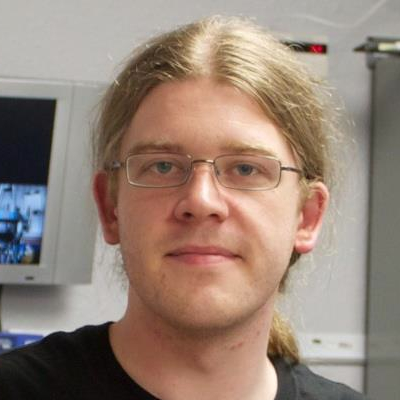
\includegraphics[width=3.6cm]{CV_Photo.jpg}
~
\section{Contact}
Department of Physics
University of Warwick
Gibbet Hill Road
Coventry
CV4 7AL
UK
~
{\bf mobile:} 
+44 7481 178055
{\bf work:} 
+44 2476 151862
{\bf email:}
{\small p.chote@warwick.ac.uk}
{\small paul@chote.net}
{\bf skype:}
{\small pchote}
~
\end{aside}

%----------------------------------------------------------------------------------------
\vspace{0.5cm}
\section{Education}
\vspace{-7mm}
\begin{entrylist}
\vspace{2mm}
\entry{}{}{Victoria University of Wellington (VUW), New Zealand}{\vspace{-0.5cm}}
\entry{2011~--~2014}{Doctor of Philosophy {\normalfont in Physics}}{}{\vspace{-0.5cm}}
\entry{2009~--~2010}{Master of Science {\normalfont in Physics with Distinction}}{}{\vspace{-0.5cm}}
\entry{2008~--~2009}{Bachelor of Science {\normalfont in Physics with Honours (1\textsuperscript{st} Class)}}{}{\vspace{-0.5cm}}
\entry{2005~--~2007}{Bachelor of Science {\normalfont in Mathematics and Physics}}{}{\vspace{-0.5cm}}
\end{entrylist}

%----------------------------------------------------------------------------------------

\section{Experience}

\begin{entrylist}
%------------------------------------------------
\entry
  {\small 2015--current}{Department of Physics, Warwick University}{Coventry, United Kingdom}
  {\jobtitle{Postdoctoral Research Fellow}\\
  I have been involved in a variety of projects during my time at Warwick, including:
  \begin{itemize}
    \item \textbf{Phantom Echoes 2 (2021~\textendash~ongoing)}\\
    Part of an international collaboration studying the launch of the Mission Extension Vehicle 2 and its docking with Intelsat 10-02 in Geostationary orbit.
    \begin{itemize}
    \item Developed and demonstrated an end-to-end procedure to observe and recover orbital custody of an object undergoing electric propulsion based on stale TLE information.
    \item Designed and undertook an extensive observation campaign to obtain a large number of high-quality light curves during the MEV-2 RPO phase.
    \item Developed reduction pipelines to extract and calibrate high-cadence single- and multi-colour photometric data.
    \end{itemize}
    \item \textbf{The threat from space debris in low earth orbit: understanding and mitigating the risk (2020~\textendash~ongoing)}\\
    Co-investigator on a successful \jobtitle{Challenge Lead Applied Systems Programme} (CLASP) project investigating new techniques for identifying and characterising space debris in Low Earth Orbit.
    \begin{itemize}
    \item Developed and installed a new robotic telescope facility.
    \item Designed and coordinated manufacture of bespoke mechanical components.
    \item Developed software control for the telescope hardware and data acquisition.
    \end{itemize}
    \item \textbf{Improving debris detection and tracking in the next generation of EU GEO monitoring sensors (2020)}\\
    Co-investigator on a successful \jobtitle{EUSST} project comparing data analysis techniques on a unique data set consisting of simultaneous small- and large-aperture telescope observations.
    \begin{itemize}
        \item Investigated morphological characteristics of tumbling debris light curves.
        \item Developed and bench-marked a proof of concept image stacking algorithm.
    \end{itemize}
    \item \textbf{GEOMON (2019~\textendash~2020)}\\
    Subcontractor on a successful \jobtitle{DASA} project developing a new concept for a Geostationary orbit monitoring system.
    \begin{itemize}
        \item Coordinated documentation and delivery of an archival data set.
        \item Iterated development and benchmarked performance of the data reduction pipelines previously developed in the \jobtitle{Precision light curves of LEO and GEO objects} project.
    \end{itemize}
    \item \textbf{Precision light curves of LEO and GEO objects (2019~\textendash~2020)}\\
    Developed observational programmes and reduction pipelines for the purpose of identifying and characterising space debris in both Low Earth Orbit (LEO) and Geosynchronous (GEO) orbits.
    \begin{itemize}
      \item Developed hardware and software upgrades to repurpose the SuperWASP North telescope for observations of LEO objects.
      \item Developed a standalone 0.36m telescope system for GEO satellite and debris observations.
      \item Developed analysis pipeline for extracting light curves from trailed images.
      \item Undertook surveys of LEO and GEO rotation rates and optical signatures.
    \end{itemize}
  \end{itemize}
}
\end{entrylist}
\begin{entrylist}
%------------------------------------------------
\entry
  {}{}{}
  {
  \begin{itemize}
    \item \textbf{Warwick One-metre telescope (2015~\textendash~ongoing)}\\
    Lead the repair and redevelopment of a 1 metre research telescope based at the Roque de Los Muchachos observatory on the Canary Island of La Palma.
    \begin{itemize}
      \item Identified optical and mechanical faults and developed repair strategies.
      \item Developed hardware and low-level software for observatory systems.
      \item Designed and implemented data management and calibration pipeline.
      \item Developed web dashboards and monitoring tools.
    \end{itemize}
    \item \textbf{Gravitational-wave Optical Transient Explorer (2015~\textendash~ongoing)}\\
    Supported the development of new optical survey telescopes based in La Palma and Australia.
    \begin{itemize}
      \item Advised on operational and safety procedures.
      \item Identified optical and mechanical faults and contributed to the development of repair strategies.
      \item Developed and maintain the common observatory weather and monitoring infrastructure.
      \item Contributed to the physical installation and ongoing hardware maintenance.
    \end{itemize}
    \item \textbf{White Dwarf Research (2015~\textendash~2018)}\\
    Involved in a range of research projects focused around White Dwarf and compact binary star systems.
    \begin{itemize}
      \item Obtained observational data using professional telescopes in Spain, Chile, New Zealand.
      \item Developed custom reduction pipelines for extracting and analysing light curves of variable objects.
      \item Identified targets of interest in wide-area astronomical surveys.
      \item Authored and contributed to refereed journal papers.
    \end{itemize}
    \item \textbf{Teaching Support (2017~\textendash~ongoing)}\\
    Tutored lab sessions for undergraduate Physics modules.
    \begin{itemize}
      \item PX150 (Physics Programming Workshop)
      \item PX277 (Computational Physics)
    \end{itemize}
  \end{itemize}
}
%------------------------------------------------
\entry
  {\small 2014--2015}{School of Chemical and Physical Sciences, VUW}{Wellington, New Zealand}
  {\jobtitle{Research Assistant: 2D X-Ray Dosimeter Development}
  \begin{itemize}
    \item Developed a 2D readout instrument for X-Ray sensitive films, adapting a 3D printer to hold a scanning laser and photon counting electronics.
    \item Characterised system properties including resolution, linearity, and noise levels.
    \item Created and characterised X-ray sensitive films in the lab.
  \end{itemize}
}
%------------------------------------------------
\entry{\small 2011~--~2014}{School of Chemical and Physical Sciences, VUW}{Wellington, New Zealand}
  {\jobtitle{PhD. Research: CCD Time-Series Photometry of White Dwarf Stars}
\begin{itemize}
    \item Developed two high-speed CCD time-series photometer instruments for use with \mbox{0.6~--~2.1\,m} research telescopes in New Zealand and the USA.
    \item Created a CCD data reduction pipeline for real-time analysis and visualisation.
    \item Acquired time-series photometry of variable white dwarf (WD) targets.
    \item Analysis of targets included identification of WD pulsation modes, investigation of pulsation stability, and the consideration of convection effects.
\end{itemize}}
%------------------------------------------------
\entry{\small 2009~--~2010}{School of Chemical and Physical Sciences, VUW}{Wellington, New Zealand}
  {\jobtitle{MSc. Research: A Semi-Analytical Model for Gravitational Microlensing}
\begin{itemize}
    \item Investigated techniques for calculating gravitational microlensing light curves.
    \item Developed and implemented a computationally efficient semi-analytical model for simulating gravitational microlensing events with up to four lens bodies.
    \item Implemented model support for orbital motion effects in the source, lens, and observer systems.
  \end{itemize}}
%------------------------------------------------
\entry{\small Summer 2008}{\small Research School of Astronomy and Astrophysics, Australian National University}{Canberra, Australia}
  {\jobtitle{Summer Scholar: RSAA Instrumentation Group}
\begin{itemize}
    \item Worked with the team commissioning a new integral field spectrograph for the 2.3\,m telescope at Siding Spring Observatory.
    \item Tested and documented an optical stimulus assembly that was used to simulate the telescope optics during instrument verification tests.
    \item Reduced archival CCD data using IRAF.
  \end{itemize}}
%------------------------------------------------
\end{entrylist}
\begin{entrylist}
%------------------------------------------------
\entry{\small Summer 2007}{School of Chemical and Physical Sciences, VUW}{Wellington, New Zealand}
  {\jobtitle{Summer Scholar: VUW Microlensing Group}
\begin{itemize}
    \item Adapted modelling code to run on University of Canterbury’s BlueFern supercomputer and the VUW Condor computing grid.
    \item Compared the benefits of the available computing resources, and determined that the best results could be obtained with the local Condor grid.
    \item Investigated the impact of three lens masses on model light curves.
  \end{itemize}}
%------------------------------------------------
\entry {\small 2007~--~2015}{School of Chemical and Physical Sciences, VUW}{Wellington, New Zealand}
  {\jobtitle{Tutoring \& Lab Development}
  \begin{itemize}
    \item Demonstrated / tutored undergraduate laboratories (usually 2 -- 10 students per session) across most of the core physics curriculum at VUW.
    \item Developed a time-series photometry experiment using a CCD camera and LEDs driven by a microcontroller to mimic variable stars.
    \item Developed a numerical simulation experiment investigating light bending around black holes and gravitational microlensing.
    \item Overhauled and modernized several existing experiments.
    \item Co-supervised research project students.
    \end{itemize}}
%------------------------------------------------
\entry{\small 2010~--~current}{Open Source Software}{}
  {\jobtitle{Core maintainer of the \href{http://www.openra.net}{OpenRA} project.}
\begin{itemize}
    \item Open source game engine recreating classic Command \& Conquer RTS titles.
    \item Designed and implemented many of the core engine systems.
    \item Performed code review and mentoring of new contributors.
	\item Performed project management, public relations, and other community roles.
	\item Member of the \jobtitle{C\&C Community Council} advising Electronic Arts and Petroglyph Games during the development of the \jobtitle{Command \& Conquer™ Remastered Collection} computer game.
  \end{itemize}}
%------------------------------------------------

\end{entrylist}

%----------------------------------------------------------------------------------------

\section{Awards}
\begin{entrylist}
\entry{\small 2018}{Merit Award}{University of Warwick}
{Award for exceptional performance during the 2017~--~2018 year.}
\entry{\small 2017}{Merit Award}{University of Warwick}
{Award for exceptional performance during the 2016~--~2017 year.}
\entry{\small 2016}{Merit Award}{University of Warwick}
{Award for exceptional performance during the 2015~--~2016 year.}
\entry{\small 2014}{Royal Society Marsden Scholarship}{Royal Society of NZ}
{Funding for tuition fees and a stipend during a 3 year PhD degree.}
\entry{}{Victoria Doctoral Completion Award}{Victoria University of Wellington}
{Awarded for successful PhD completion within the scheduled time allocation.}
\entry{\small 2009}{Victoria Master's Scholarship}{Victoria University of Wellington}
{Awarded based on academic merit to fund tuition fees and a stipend during a 1 year masters degree.}
\entry{\small 2008}{VUW Graduate Award}{Victoria University of Wellington}
{Awarded on the basis of academic merit to support graduate degree study.}
\vspace{-3mm}\entry{}{Mike Collins Scholarship in Physics}{Victoria University of Wellington}{}
\vspace{-3mm}\entry{\small 2005}{Ormond Wilson Scholarship}{Victoria University of Wellington}{}
\entry{}{J Mills Family Scholarship}{J Mills Family Trust}
{Award for Dux of Karamu High School in 2004.}
\end{entrylist}


%----------------------------------------------------------------------------------------
\pagebreak

\section{Publications}
{\bf First-author refereed publications:}\\
~\vspace{-2mm}\\
\begin{entrylist}
  \entry{\small 2021}{\small NGTS and HST insights into the long-period modulation in GW Librae }{}
  {\small Chote, P., et al. 2021, MNRAS, 502, 581. \textsc{DOI:}\href{http://dx.doi.org/10.1093/mnras/staa4015}{10.1093/mnras/staa4015}}
  \entry{\small 2016}{\small The post-outburst pulsations of the accreting white dwarf in the cataclysmic variable GW Librae}{}
  {\small Chote, P., and Sullivan, D.J. 2016, MNRAS, 458, 1393. \textsc{DOI:}\href{http://dx.doi.org/10.1093/mnras/stw421}{10.1093/mnras/stw421}}

  \entry{\small 2014}{\small Puoko-nui: a flexible high-speed photometric system}{}
  {\small Chote, P., et al. 2014, MNRAS, 440, 1490. \textsc{DOI:}\href{http://dx.doi.org/10.1093/mnras/stu348}{10.1093/mnras/stu348}}
  
  \entry{\small 2013}{\small Time series photometry of the helium atmosphere pulsating white dwarf EC 04207-4748}{}
  {\small Chote, P., et al. 2013, MNRAS, 431, 520. \textsc{DOI:}\href{http://dx.doi.org/10.1093/mnras/stt180}{10.1093/mnras/stt180}}
\end{entrylist}\\

{\bf Selected co-authored refereed publications:}\\
~\vspace{-2mm}\\
\begin{entrylist}
  \entry{\small 2021}{\small DebrisWatch I: A survey of faint geosynchronous debris}{}
  {\small Blake, J. A., et al. 2021, AdSpR, 67, 360. \textsc{DOI:}\href{http://dx.doi.org/10.1016/j.asr.2020.08.008}{10.1016/j.asr.2020.08.008}}
  
  \entry{}{\small The Pulsating White Dwarf G117-B15A: Still the Most Stable Optical Clock Known}{}
  {\small Kepler, S. O., et al. 2021, ApJ, 906, 7. \textsc{DOI:}\href{http://dx.doi.org/10.3847/1538-4357/abc626}{10.3847/1538-4357/abc626}}

  \entry{\small 2020}{\small An ultra-massive white dwarf with a mixed hydrogen-carbon atmosphere as a likely merger remnant }{}
  {\small Hollands, M. A., et al. 2020, NatAs, 4, 633. \textsc{DOI:}\href{http://dx.doi.org/10.1038/s41550-020-1028-0}{10.1038/s41550-020-1028-0}}

  \entry{}{\small V1460 Her: a fast spinning white dwarf accreting from an evolved donor star }{}
  {\small Ashley, R. P., et al. 2020, MNRAS, 499, 149. \textsc{DOI:}\href{http://dx.doi.org/10.1093/mnras/staa2676}{10.1093/mnras/staa2676}}

  \entry{\small 2019}{\footnotesize The PDS 110 observing campaign - photometric and spectroscopic observations reveal eclipses are aperiodic}{}
  {\small Osborn, H. P., et al. 2019, MNRAS, 485, 1614. \textsc{DOI:}\href{http://dx.doi.org/10.1093/mnras/stz283}{10.1093/mnras/stz283}}

  \entry{}{\small Multiwavelength observations of the EUV variable metal-rich white dwarf GD 394}{}
  {\small Wilson, D. J., et al. 2019, MNRAS, 483, 2941. \textsc{DOI:}\href{http://dx.doi.org/10.1093/mnras/sty3218}{10.1093/mnras/sty3218 }}

  \entry{\small 2018}{\small The Next Generation Transit Survey (NGTS)}{}
  {\small Wheatley, P. J., et al. 2018, MNRAS, 475, 4476. \textsc{DOI:}\href{http://dx.doi.org/10.1093/mnras/stx2836}{10.1093/mnras/stx2836}}

  \entry{}{\small VLA radio observations of AR Scorpii}{}
  {\small Stanway, E. R., et al. 2018, A\&A, 611, 66. \textsc{DOI:}\href{http://dx.doi.org/10.1051/0004-6361/201732380}{10.1051/0004-6361/201732380}}

  \entry{\small 2017}{\small Multiband photometry and spectroscopy of an all-sky sample of bright white dwarfs}{}
  {\small Raddi, R., et al. 2017, MNRAS, 472, 4173. \textsc{DOI:}\href{http://dx.doi.org/10.1093/mnras/stx2243}{10.1093/mnras/stx2243}}

  \entry{}{\footnotesize White Dwarf Rotation as a Function of Mass and a Dichotomy of Mode Line Widths: Kepler Observations of 27 Pulsating DA White Dwarfs through K2 Campaign 8}{}
  {\small Hermes, J. J., et al. 2017, ApJS, 232, 23. \textsc{DOI:}\href{http://dx.doi.org/10.3847/1538-4365/aa8bb5}{10.3847/1538-4365/aa8bb5}}

  \entry{\small 2016}{\footnotesize High-speed Photometry of the Disintegrating Planetesimals at WD1145+017: Evidence for Rapid Dynamical Evolution}{}
  {\small Gänsicke, B. T., et al. 2016, ApJ, 829, 82. \textsc{DOI:}\href{http://dx.doi.org/10.3847/2041-8205/818/1/L7}{10.3847/2041-8205/818/1/L7}}

\entry{}{\small Outbursts in Two New Cool Pulsating DA White Dwarfs}{}
  {\small Bell, K. J., et al. 2016, ApJ, 818, L7. \textsc{DOI:}\href{http://dx.doi.org/10.3847/0004-637X/829/2/82}{10.3847/0004-637X/829/2/82}}

\entry{\small 2015}{\small Insights into internal effects of common-envelope evolution using the extended Kepler mission}{}
  {\small Hermes, J. J., et al. 2015, MNRAS, 451, 1701. \textsc{DOI:}\href{http://dx.doi.org/10.1093/mnras/stv1053}{10.1093/mnras/stv1053}}

\entry{}{\small A Second Case of Outbursts in a Pulsating White Dwarf Observed by Kepler}{}
  {\small Hermes, J. J., et al. 2015, ApJ, 810, L5. \textsc{DOI:}\href{http://dx.doi.org/10.1088/2041-8205/810/1/L5}{10.1088/2041-8205/810/1/L5}}

\entry{\small 2014}{\small Radius constraints from high-speed photometry of 20 low-mass white dwarf binaries}{}
  {\small Hermes, J. J., et al. 2014, ApJ, 792, 39. \textsc{DOI:}\href{http://dx.doi.org/10.1088/0004-637X/792/1/39}{10.1088/0004-637X/792/1/39}}

\entry{}{\small Found: the progenitors of AM CVn and supernovae .Ia}{}
  {\small Kilic, M., et al. 2014, MNRAS, 439, L26. \textsc{DOI:}\href{http://dx.doi.org/10.1093/mnrasl/slt151}{10.1093/mnrasl/slt151}}

\entry{\small 2012}{\footnotesize HST and Optical Data Reveal White Dwarf Cooling, Spin, and Periodicities in GW Librae 3-4 Years after Outburst}{}
  {\small Szkody, P., et al. 2012, ApJ, 753, 158. \textsc{DOI:}\href{http://dx.doi.org/10.1088/0004-637X/753/2/158}{10.1088/0004-637X/753/2/158}}
\end{entrylist}

\vspace{-4mm}{\small Full list available at \url{http://adsabs.harvard.edu/cgi-bin/basic_connect?qsearch=Chote\%2C+P}}\\
\\
\pagebreak\\
{\bf Conference Presentations:}\\
~\vspace{-2mm}\\
\begin{entrylist}

\entry{\small 2021}{\small MEV-2 RPO Observation Campaign}{Oral Presentation}
{\small PHANTOM ECHOES 2 Post-Campaign Workshop, Virtual}

\entry{\small 2020}{\small Understanding the optical variability in light curves of objects in Low Earth Orbit}{Oral Presentation}
{\small Physics of Remote Sensing Program Review, Virtual}

\entry{}{\small Precision Optical Light Curves of LEO and GEO Objects}{Oral Presentation}
{\small GNOSIS Precision SSA Workshop, Virtual}

\entry{\small 2019}{\small Precision Optical Light Curves of LEO and GEO Objects}{Poster}
{\small Advanced Maui Optical and Space Surveillance Technologies Conference 2019, Hawaii, USA}

\entry{\small 2018}{\small Ongoing Observational Projects}{Oral Presentation}
{\small Astrodynamics Community of Interest Meeting \#12, London, UK}

\entry{\small 2017}{\small GW Librae in NGTS}{Oral Presentation}
{\small NGTS Project Meeting, Leicester, UK}

\entry{\small 2016}{\small The post-outburst pulsations of GW Librae}{Oral Presentation}
{\small 20th European White Dwarf Workshop, Warwick, UK}

\entry{}{\small The Warwick one-metre telescope}{Poster}
{\small 20th European White Dwarf Workshop, Warwick, UK}

\entry{\small 2012}{\small New Time-Series Observations of the Intriguing Object GW Librae}{Oral Presentation}
{\small 18th European White Dwarf Workshop, Krakow, Poland}

\entry{}{\small The Puoko-nui CCD Time-Series Photometer}{Poster}
{\small 18th European White Dwarf Workshop, Krakow, Poland}

\entry{\small 2011}{\small High precision CCD time-series photometry}{Oral Presentation}
{\small Royal Astronomical Society Conference, Wellington, NZ}

\entry{}{\small Time Series Photometry of Pulsating White Dwarf Stars}{Oral Presentation}
{\small New Zealand Institute of Physics Conference, Wellington, NZ}
\end{entrylist}
%----------------------------------------------------------------------------------------
{\bf Other publications:}\\
~\vspace{-2mm}\\
\begin{entrylist}
  \entry{\small 2019}{\small Precision Optical Light Curves of LEO and GEO Objects}{}
  {\small Chote, P., Blake, J. A., Pollacco, D, Technical Paper.\\
  \url{https://ui.adsabs.harvard.edu/abs/2019amos.confE..52C}}
  
  \entry{\small 2015}{\small Simulating the photometric study of pulsating white dwarf stars in the physics laboratory}{}
  {\small Chote, P., and Sullivan, D.J. 2015.\\
  \url{https://arxiv.org/abs/1502.01767}}

  \entry{\small 2014}{\small CCD Time-Series Photometry of White Dwarf Stars}{}
  {\small Chote, P. 2014, PhD. Thesis, Victoria University of Wellington.\\
  \url{http://researcharchive.vuw.ac.nz/handle/10063/3512}}

  \entry{\small 2011}{\small A Semi-Analytical Model for Gravitational Microlensing}{}
  {\small Chote, P. 2011, MSc. Thesis, Victoria University of Wellington.\\ \url{http://researcharchive.vuw.ac.nz/ handle/10063/1890}}
\end{entrylist}
\section{References}
{\small Available on request.}
\end{document}

\section{Selected Software Projects}
%------------------------------------------------

\parbox[t]{12.8cm}{%
    \textbf{Warwick one-metre observatory software}%
    \hfill%
    {\footnotesize\color{lightgray} \faGithub~~\url{https://github.com/warwick-one-metre/}}\\%
    A collection of microservices and utilities that make up the control systems for the Warwick one-metre telescope at the Roque de los Muchachos observatory on La Palma.  Low level daemons provide a standardized software interface (using Pyro remote procedure calls) to the hardware components, with higher level daemons implementing logic for environmental monitoring and observatory operation.  Real time image analysis feeds back into the closed-loop telescope control system.
    \vspace{\parsep}\\
    Core Skills:
    \begin{itemize}
      \item Python development.
      \item Designing fault tolerant systems.
      \item Integrating software with complex hardware environments.
      \item Designing and deploying microservices.
      \item Real time data analysis.
    \end{itemize}
}

%------------------------------------------------
%\parbox[t]{12.8cm}{%
%    \textbf{NGTS transient object detection pipeline}%
%    \hfill%
%    {\small\color{lightgray} \faGithub~~\url{https://github.com/pchote/ngtransients/}}\\%
%    A data-driven image analysis pipeline for detecting transient events and variable stars in the \italica{Next Generation Transit Survey}.  Currently under development and targeting the archive of historical data, but is designed for future observatory deployment to run in real time and drive automatic alerts for followup by other facilities.
%    \vspace{\parsep}\\
%    Core Skills:
%    \begin{itemize}
%      \item Python development (including numpy and matplotlib).
%      \item Working with large data sets.
%      \item Performance sensitive software design and implementation.
%      \item Distributed computing (Sun/Oracle Grid Engine).
%    \end{itemize}
%}

%------------------------------------------------

\parbox[t]{12.8cm}{%
    \textbf{OpenRA}%
    \hfill%
    {\small\color{lightgray} \faGithub~~\url{https://github.com/OpenRA/OpenRA/}}\\%
    A cross-platform GPL3 real time strategy engine for building games in the style of the classic 2D/2.5D Command \& Conquer titles.  Community driven recreations of \italica{Command \& Conquer}, \italica{Red Alert}, and \italica{Dune 2000}~have a thriving online player base.
    \vspace{\parsep}\\
    Core Skills:
    \begin{itemize}
        \item Advanced C\# development (including LINQ, P/Invoke, reflection, codegen).
        \item OpenGL development.
        \item Gameplay and user interface design.
        \item Project management.
        \item Code review and mentoring.
        \item Continuous integration and deployment using Travis CI.
        \item Triaging user feedback and bug reports into actionable tasks.
        \item Web development and maintenance (PHP, Ruby, SQLite, HTML/Javascript/CSS).
    \end{itemize}
}

%------------------------------------------------

\parbox[t]{12.8cm}{%
    \textbf{Puoko-nui time-series photometer}%
    \hfill{\small\color{lightgray} \parbox{6.4cm}{\faGithub~~\url{https://github.com/pchote/Puoko-nui/} \\ \faGithub~~\url{https://github.com/pchote/Karaka/}}}\\%
    Instrument control software for the Puoko-nui astronomical photometer instrument.  Interfaces with a frame-transfer CCD camera and GPS receiver to enable high-speed image acquisition with precise absolute timing information for observing variable astronomical phenomena.
    \vspace{\parsep}\\
    Core Skills:
    \begin{itemize}
      \item C development.
      \item Linux kernel driver development / maintenance.
      \item Embedded C development (AVR microcontroller).
      \item Designing real-time systems.
      \item Integrating software with complex hardware environments.
    \end{itemize}
}\\

{More projects with source code available at \url{https://github.com/pchote/}\vspace{5mm}}\\
\vspace{-0.5cm}
%----------------------------------------------------------------------------------------
\section{References}
{\small Available on request.}
\end{document}

\section{Links}
{\small \faLinkedin~linkedin.com/in/pchote}
{\small \faGithub~github.com/pchote}
~
\section{Computing}
\vspace{1mm}{\bf Operating systems:} 
{\small Linux, macOS, Windows}
\vspace{1mm}{\bf Programming Languages:} 
{\small C, C\#, Python, Bash,\\HTML, CSS, Javascript}
\vspace{1mm}{\bf Display APIs:} 
{\small OpenGL, PGPLOT, Matplotlib, Flot}
\vspace{1mm}{\bf Embedded Systems:}
{\small AVR, ARM}
\vspace{1mm}{\bf Web Frameworks:}
{\small Flask, Django, JQuery, Bootstrap}
\vspace{1mm}{\bf Grid Computing:} 
{\small SGE, Condor, DRMAA}
\vspace{1mm}{\bf Version Control:} 
{\small Git, SVN}
\vspace{1mm}{\bf Word Processing:} 
{\small \LaTeX, Microsoft Office}
~